%acmsmall: The default journal template style.
%acmlarge: Used by JOCCH and TAP.
%acmtog: Used by TOG.
%acmconf: The default proceedings template style.
%sigchi: Used for SIGCHI conference articles.
%sigchi-a: Used for SIGCHI ``Extended Abstract'' articles.
%sigplan: Used for SIGPLAN conference articles.
\documentclass[format=acmtog,12pt,screen=true,review=false,natbib=false,]{acmart}

%% \BibTeX command to typeset BibTeX logo in the docs
%\AtBeginDocument{%
%  \providecommand\BibTeX{{%
%    \normalfont B\kern-0.5em{\scshape i\kern-0.25em b}\kern-0.8em\TeX}}}

%% Rights management information.  This information is sent to you
%% when you complete the rights form.  These commands have SAMPLE
%% values in them; it is your responsibility as an author to replace
%% the commands and values with those provided to you when you
%% complete the rights form.
\setcopyright{acmcopyright}
\copyrightyear{2019}
\acmYear{2019}
\acmDOI{123456789}

%%
%% These commands are for a JOURNAL article.
\acmJournal{TOMACS}
\acmVolume{1}
\acmNumber{1}
\acmArticle{1}
\acmMonth{1}

%%
%% Submission ID.
%% Use this when submitting an article to a sponsored event. You'll
%% receive a unique submission ID from the organizers
%% of the event, and this ID should be used as the parameter to this command.
\acmSubmissionID{123-456-789}

%% Useful packages
\usepackage{multicol}
%\usepackage[UKenglish]{babel}
\usepackage{comment}
\usepackage{textcomp}
\usepackage{tabu}
\usepackage{caption}
\usepackage[scaled]{helvet}
\usepackage[T1]{fontenc}
\usepackage[utf8]{inputenc}
\usepackage{sansmath}
\usepackage{textpos}
\usepackage{ifxetex}
\usepackage{stackengine}
\usepackage{tabularx,longtable,multirow,subfigure,caption} %hang caption
\usepackage{fncylab} %formatting of labels
\usepackage{fancyhdr}
\usepackage{color}
\usepackage[ugly]{units}
\usepackage{url}
\usepackage{float}
\usepackage{csquotes}
\usepackage[english]{babel}
\usepackage{amsmath}
\usepackage{bm}
\usepackage{mathtools}
\DeclarePairedDelimiter\ceil{\lceil}{\rceil}
\DeclarePairedDelimiter\floor{\lfloor}{\rfloor}
\usepackage{graphicx}
\usepackage[colorinlistoftodos]{todonotes}
\usepackage{epstopdf} % automatically replace .eps with .pdf in graphics
%\usepackage{backref}
\usepackage{array}
\usepackage{latexsym}
\usepackage{etoolbox}
\usepackage{enumerate} % for numbering with [a)] format 
\usepackage{enumitem}
\usepackage{tablefootnote}
\usepackage{booktabs}
\usepackage{tcolorbox}
\usepackage{silence}
\usepackage{multicol}
%\usepackage{natbib}
\usepackage{multirow}
\usepackage{pbox, cellspace}
\cellspacetoplimit = 6pt
\cellspacebottomlimit = 12pt

\usepackage[style=ACM-Reference-Format,backend=biber,backref=true,hyperref=true,giveninits=true,maxbibnames=999,sorting=none,citestyle=numeric,sortcites]{biblatex} 
\WarningFilter{biblatex}{Patching footnotes failed}



%% The majority of ACM publications use numbered citations and
%% references.  The command \citestyle{authoryear} switches to the
%% "author year" style.
%% If you are preparing content for an event
%% sponsored by ACM SIGGRAPH, you must use the "author year" style of
%% citations and references.
%\citestyle{acmauthoryear}
%\citestyle{acmnumeric}
%\citestyle{acmauthoryear}

\addbibresource{Bib.bib}
\usepackage{hyperref} % provide links in pdf
\hypersetup{
  pdftitle={},
  pdfsubject={}, 
  pdfauthor={},
  pdfkeywords={}, 
  pdfstartview=FitH,
  pdfpagemode={UseOutlines},
  bookmarksnumbered=true, 
  bookmarksopen=true, 
  colorlinks=true, 
  citecolor=blue,
  filecolor=blue, 
  linkcolor=blue, 
  urlcolor=blue,
  hypertexnames=true,
  breaklinks=true}

%%
%% The "title" command has an optional parameter,
%% allowing the author to define a "short title" to be used in page headers.
\title[Implementing a hyper-elastic material law ]{Dynamic Impact Response of Laminated Window Glass}

%If your title is lengthy, you must define a short version to be used
%in the page headers, to prevent overlapping text. The \texttt{title}
%command has a ``short title'' parameter:

%%
%% The "author" command and its associated commands are used to define
%% the authors and their affiliations.
%% Of note is the shared affiliation of the first two authors, and the
%% "authornote" and "authornotemark" commands
%% used to denote shared contribution to the research.

%If your author list is lengthy, you must define a shortened version of
%the list of authors to be used in the page headers, to prevent
%overlapping text. The following command should be placed just after
%the last \texttt{\author{}} definition:
%\begin{verbatim}
%  \renewcommand{\shortauthors}{McCartney, et al.}
%\end{verbatim}
%Omitting this command will force the use of a concatenated list of all
%of the authors' names, which may result in overlapping text in the
%page headers.

\author{John-Paul Latham}
\authornote{Imperial College London.}
\email{j.p.latham@imperial.ac.uk}

\author{Jason Xiang}
\authornotemark[1]
\email{j.xiang@imperial.ac.uk}

\author{Ado Farsi}
\authornotemark[1]
\email{ado.farsi@imperial.ac.uk}

\author{Michael Trapp}
\email{mt5918@ic.ac.uk}
\orcid{1234-5678-9012}
\authornotemark[1]

%%
%% By default, the full list of authors will be used in the page
%% headers. Often, this list is too long, and will overlap
%% other information printed in the page headers. This command allows
%% the author to define a more concise list
%% of authors' names for this purpose.
\renewcommand{\shortauthors}{Latham et al.}

%% end of the preamble, start of the body of the document source.
\begin{document}

%%
%% The abstract is a short summary of the work to be presented in the
%% article.
\begin{abstract}
    Deliberate acts of terrorism, criminal activity and malicious behaviour pose a national threat to buildings and infrastructure. A recent state-of the arts review by \texttt{EU} decision makers revealed that current building guidelines tend to not take these threats into account, see \cite{Sto15}. To update these guidelines, accurate numerical models are required to quantify the resilience of building elements against explosions.

    \bigbreak
    The Applied Modelling and Computation Group (\texttt{AMCG}) at Imperial College London has recently developed a novel coupled dynamic gas/solid \texttt{FEMDEM} code and applied it successfully to geological and biological applications. In this paper, the code is applied to simulate \texttt{2D} and \texttt{3D} projectile impact on a single laminate. In the future, the software will be used to simulate shock wave impact on secondary laminated glass.
    
    \bigbreak
    practical importance
\end{abstract}

%%
%% The code below is generated by the tool at http://dl.acm.org/ccs.cfm.
%% Please copy and paste the code instead of the example below.
%%
%\section{CCS Concepts and User-Defined Keywords}
%
%Two elements of the ``acmart'' document class provide powerful
%taxonomic tools for you to help readers find your work in an online
%search.
%
%The ACM Computing Classification System ---
%\url{https://www.acm.org/publications/class-2012} --- is a set of
%classifiers and concepts that describe the computing
%discipline. Authors can select entries from this classification
%system, via \url{https://dl.acm.org/ccs/ccs.cfm}, and generate the
%commands to be included in the \LaTeX\ source.

\begin{CCSXML}
<ccs2012>
<concept>
<concept_id>10010405.10010432.10010439</concept_id>
<concept_desc>Applied computing~Engineering</concept_desc>
<concept_significance>300</concept_significance>
</concept>
</ccs2012>
\end{CCSXML}
\ccsdesc[300]{Applied computing~Engineering}

%%
%% Keywords. The author(s) should pick words that accurately describe
%% the work being presented. Separate the keywords with commas.
\keywords{Laminated Window Glass, Impact Response, ACMG, Imperial College, Computational Modelling, Numerical Modelling, FEMDEM, Combined Discrete-Finite Element Method, Coupled Physics Model, Multi-Phase Model, Multi-Physisc Model, Brittle Materials, Crack Initiation, Crack Propagation, Fracturing}
%%
%% This command processes the author and affiliation and title
%% information and builds the first part of the formatted document.

\maketitle

\section{Physics Theory}
\label{sec:PhysicsTheory}

\subsection{Laminated Glass Model}

%Picture of Laminated Glass
%Measurements of the plies and inter-layer

Laminated glass is a sandwich structure consisting of two brittle glass plies and an adhered visco-elastic polymer inter-layer (or inter-face) in between. The bonding between the glass and the inter-layer is without physical adhesive \cite{Sam19}. Secondary laminated glass consists of two such laminates, separated by a layer of air.

\bigbreak
Advantageous properties of laminated glass include a relatively high penetration resistance \cite{Xu14}, low weight \cite{Wu14} and the adherence of fractured glass fragments to the structure to reduce the risk of injuries\cite{Xu14, Che17, Flo98, Ji98}. Breakage of the inner ply significantly reduces strength and facilitates a full collapse of the glass \cite{Flo98}. An optional back layer (usually poly-carbonate (\texttt{PC}) \cite{Bra10, Mon04}) improves structural stability and additional energy absorption \cite{Bio10, Bra10}.

\bigbreak
The prediction of crack initiation and propagation poses a significant challenge and requires ongoing research effort. 

\bigbreak
Local stress intensification is caused by pre-existing micro-structural material flaws (inhomogeneities or discontinuities) such as micro-cracks and voids \cite{Sch12}. 

\bigbreak
Many fracture models have been proposed. This paper uses a local combined single and smeared crack model approach \cite{Mun99, Lat15}. In this approach, a single crack is replaced by a blunt crack band \cite{Mun04}.

\begin{figure}[!htbp]
    \centering
    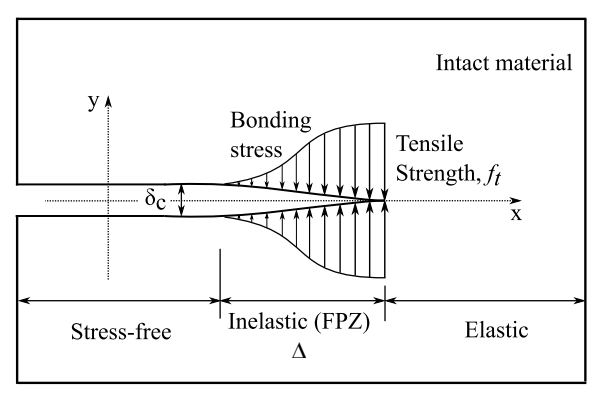
\includegraphics[width=\columnwidth]{LaminatedGlassProjectile/finalreport/Dugdale.PNG}
    \caption{Single Crack (Dugdale) Model. \cite{Abu15}}
    \label{fig:dugdale}
\end{figure}

\bigbreak
The single crack model in Fig. \ref{fig:dugdale} assumes the crack tip is located in a fracture process zone (\texttt{FPZ}). Plastic bonding stress $\sigma\leq f_{\rm{t}}$ causes the crack tip to open up, up to a critical separation length $\delta=\delta_{\rm{c}}$ \cite{Abu15}. 

\bigbreak
The \texttt{Y} code contains the Mohr-Coulomb constitutive model \cite{Lat15}, described by

\begin{equation}
    \label{eq:MohrCoulomb}
    \tau=c+\sigma\,{\rm{tan}}\phi\,,
\end{equation}

with shear stress $\tau$, normal stress $\sigma$, internal cohesion $c$ and internal friction angle $\phi$. The internal friction coefficient is given by

\begin{equation}
    \label{eq:intfriccoeff}
    \eta={\rm{tan}}\phi
\end{equation}

The stresses $\sigma$ and $\tau$ correspond to normal and shear displacements $\delta_{\rm{n}}$ and $\delta_{\rm{s}}$ and tensile and shear strengths $f_{\rm{t}}$ and $f_{\rm{s}}$. The material strengths are defined as the maximum strength in the stress-displacement diagram (Fig. \ref{fig:FractureEnergy}), with maximum elastic displacement $\delta_{\rm{p}}$ and critical displacement $\delta_{\rm{s}}$.

\begin{figure}[!htbp]
    \centering
    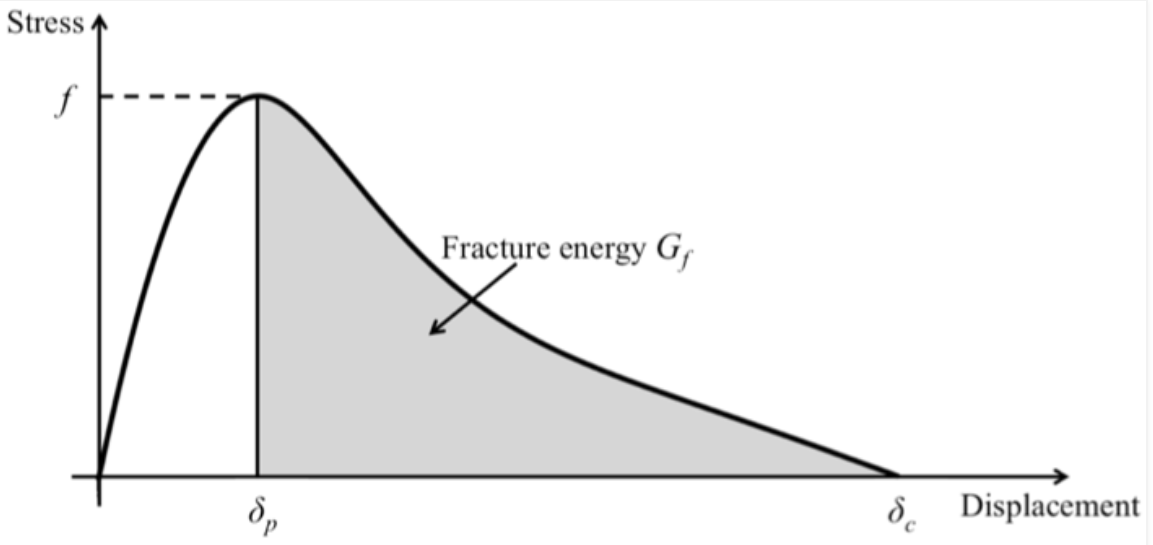
\includegraphics[width=\columnwidth]{FractureEnergy}
    \caption{Stress-displacement curve according to the single and smeared crack model. \cite{Lat15}}
    \label{fig:FractureEnergy}
\end{figure}

The fracturing in the strain-softening part is modelled using joint elements which are generated between two neighbouring shell elements. Cracks coincide with the element edges \cite{Abu15}.

\bigbreak
Detailed descriptions are given by Latham et al \cite{Lat15}, Munjiza et al \cite{Mun04}, Lei et al \cite{Lei16} and Chen and Chang \cite{Che18}.

\subsection{Inter-layer Model}

The task of the inter-layer is the absorption of impact energy and the maintenance of adhesion to the plies \cite{Wu14}. The inter-layer consists of one or more sheets. Common inter-layer materials include polymers such as polyvinyl butyral (\texttt{PVB}), thermoplastic polyurethane (\texttt{TPU}), and most recently \texttt{SentryGlas}\textregistered Plus (\texttt{SGP}) \cite{Moh18, Wan18}. 

\bigbreak
Mechanical properties of the inter-layer are dependent on the fracture state of the laminated glass \cite{Kun15}. Prior to fracture, straining of the inter-layer is limited, permitting the application of linear visco-elastic laws. After the failure of the glass, the inter-layer is subject to large strains and linear visco-elasticity is no longer applicable. Instead, the inter-layer is modelled as a hyper-elastic material \cite{Gha15, Kim15}. Work done by stresses onto such materials only depends on the reference state $X$ and the current state $x$, but not on the load path (Fig. \ref{fig:deformation}). Deformation from $X$ to $x$ is described by a deformation gradient \cite{Gu07}

\begin{equation}
    \label{eq:defgrad}
    F = \frac{{\rm{d}}\varphi}{{\rm{d}}X}
\end{equation}

with mapping function $\varphi$ mapping from $X$ to $x$.

\begin{figure}[!htbp]
    \centering
    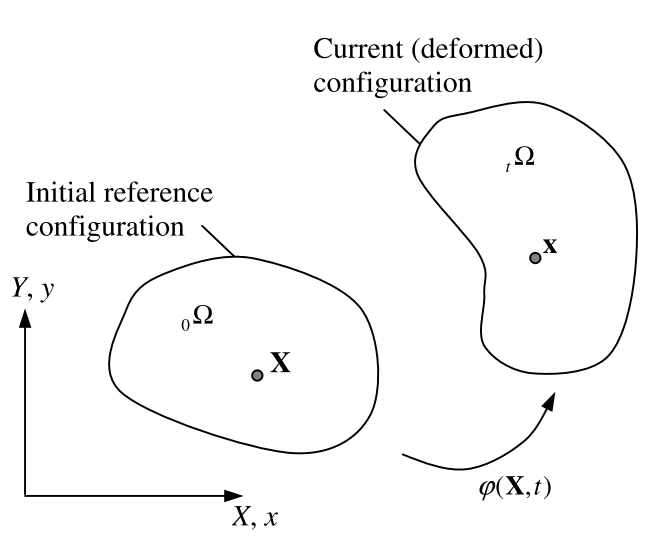
\includegraphics[width=\columnwidth]{Deformation}
    \caption{Deformation from reference to current state. \cite{Gu07}}
    \label{fig:deformation}
\end{figure}

Hyper-elastics are mathematically described by a characteristic strain energy density function $W$. One of the simplest hyper-elastic models is the \texttt{Neo-Hookean} model \cite{Gha15} whose characteristic function is given by

\begin{equation}
    \label{eq:NeoHooke}
    W=\frac{\mu_{\rm{0}}}{2}\left(I_{\rm{1}}-3\right)-\mu_{\rm{0}}\,{\rm{ln}}\,J+\frac{\lambda_{\rm{0}}}{2}{\rm{ln}}^2\,J\,,
\end{equation}

with Lam\'{e} constants $\lambda_{\rm{0}}$ and $\mu_{\rm{0}}$ from the linearised theory, $J=\lvert F\rvert$ and first invariant $I_{\rm 1}=C_{\rm{II}}$ with right Cauchy stress tensor \cite{Gha15}

\begin{equation}
    C_{\rm{ij}}=F_{\rm{Ii}}\,F_{\rm{Ij}}\,.
\end{equation}

Upper case indices refer to the reference configuration, while lower case indices refer to the current configuration.

\bigbreak
Another common, simple hyper-elastic model is the \texttt{Mooney - Rivlin} model \cite{Aba13, Kum16}. The characteristic strain energy function for the compressible 2-Parameter \texttt{Mooney - Rivlin} model \cite{Kum16} is given by

\begin{equation}
    \label{eq:MooneyRivlinSEF}
    W_{\rm{2}} = C_{\rm{10}}\left(\bar{I}_{\rm{1}}-1\right)+C_{\rm{01}}\left(\bar{I}_{\rm{2}}-1\right)+\frac{1}{d}\,(J-1)\,,
\end{equation}

where $C_{\rm{10}}$ and $C_{\rm{01}}$ are adjustable parameters, $d=2\,/\,K$ with bulk modulus $K$ and $\bar{I}_{\rm{1}}=J^{-\frac{1}{3}}\,I_{\rm{1}}$ and $\bar{I}_{\rm{2}}=J^{-\frac{1}{3}}\,I_{\rm{2}}$ are deviatoric invariants \cite{Aba13}. The second invariant is given by

\begin{equation}
    I_{\rm{2}}=\frac{1}{2}\left(C^2_{JJ}-C_{IK}C_{KI}\right)\,.
\end{equation}

\bigbreak
Other hyper-elastic models \cite{Aba13} include a more general polynomial model, \texttt{Arruda-Boyce}, \texttt{Ogden} and \texttt{Yeoh}. For the polynomial model, customized coefficients \cite{Sam19} already exist in the literature, specifically for laminated glass.

\bigbreak
Modelling the occurence of fracture needs to be permitted for the inter-layer as well, as fracturing of the inter-layer is possible. This consideration necessitates the extension of the smeared single and combined fracture model to the inter-layer.

\section{Numerical Modelling Theory}
\label{sec:NumericsTheory}

\subsection{FEMDEM Model}
The combined finite-discrete element method, \texttt{FEMDEM} or \texttt{FDEM}, contains bodies is represented by a discrete element that interacts with neighbouring discrete elements . In addition, each discrete element is discretised into finite elements. Each discrete element has its own finite element mesh. Each finite element mesh employed captures the deformability of a discrete element. Each discrete element is discretised into finite elements. Fracture and fragmentation processes are in essence processes of transition from continua to discontinua. It is also in principle possible to imagine an inverse process of particles merging together.\cite{Mun04}

\bigbreak
The combined discrete finite element method \texttt{FEMDEM} \cite{Wan18, Mun95, Mun99, Mun04, Mun12, Mun13, Guo16, Gao14, Xu14, Che18} is able to model the detection, interaction, deformation and fracturing of matrix bodies. These bodies are modelled as discrete elements, each consisting of a cluster of finite elements. Fracturing results in the formation of new discrete elements \cite{Mun13}.

\bigbreak
Based on the \texttt{3D} \texttt{FDEM} code \texttt{Y3D} by Munjiza et al \cite{Mun95, Mun99, Mun04}, Xiang et al \cite{Xia09} added many detailed improvements and features to the code. The new model, \texttt{Solidity}, is capable of creating realistic coupled multi-physics simulations. In contrast to conventional models, Solidity is not reliant on element deformability restriction constraints (due to the locking problem) and uses simpler triangular, quadratic and tetrahedral elements \cite{Lat15}. 

\subsection{Governing Equations}

The governing equations for the finite element calculations in the \texttt{FEMDEM} method are the equations of motion. The equations are given by

\begin{equation}
    M\ddot{x}+\mu\dot{x}+f_{\rm{int}}=f_{\rm{ext}}=f_{\rm{l}}+f_{\rm{b}}+f_{\rm{c}}\,,
\end{equation}

with lumped nodal mass matrix $M$, nodal displacements $x$, viscosity $\mu$, internal nodal forces $f_{\rm{int}}$ and external nodal forces $f_{\rm{ext}}$. External forces contain consist of external loads $f_{\rm{l}}$, bonding forces $f_{\rm{b}}$ and contact forces $f_{\rm{c}}$. Internal forces $f_{\rm{int}}$ are generated by element deformation. \texttt{FEMDEM} systems solve these equations via explicit time integration using the forward \texttt{Euler} method \cite{Lei16}.

\subsection{Contact Detection}

The combination of discrete and finite elements is established via an interaction algorithm \cite{Lei16}. This algorithm consists of contact detection \cite{Che15} and contact interaction \cite{Mun13}. Contact detection is carried out using search algorithms. 

\bigbreak
Contact detection is aimed at detecting couples of discrete elements close to each other, i.e. eliminating couples of discrete elements that are far from each other and cannot possibly be in contact. In other words, contact detection is aimed at avoiding processing contact interaction when there is no contact. In that sense, contact detection is aimed at reducing \texttt{CPU} requirements, i.e. reducing processing (run) times. \cite{Mun04}

\bigbreak
Contact interaction is only considered for discrete elements which are within a buffer size $b$ of each other, given by

\begin{equation}
    \label{eq:buff}
    b = 0.1\,\Delta_{\rm{min}}\,,
\end{equation}

where $\Delta_{\rm{min}}$ is the minimum edge\footnote{minimum element side length, minimum size}.

\subsection{Contact Interaction}

Penetration of a contractor\footnote{index c} body into a target\footnote{index t} body is implemented in the \texttt{Y} code by the \texttt{potential contact force method}, see Fig. \ref{fig:contact} \cite{Mun04}. Assumption of a conservative force field enables the following description of the contact forces,

\begin{align}
    f_{\rm{c}}^{\rm{2D}}&=-f_{\rm{t}}^{\rm{2D}}=\oint_{\Gamma_{\beta{\rm{t}}\cap\beta{\rm{c}}}}n_{\Gamma}\left(\varphi_{\rm{c}}-\varphi_{\rm{t}}\right)\,{\rm{d}}\Gamma\,,\\
    f_{\rm{c}}^{\rm{3D}}&=-f_{\rm{t}}^{\rm{3D}}=\int_{S_{\beta{\rm{t}}\cap\beta{\rm{c}}}}n_{S}\left(\varphi_{\rm{c}}-\varphi_{\rm{t}}\right)\,{\rm{d}}S\,,
\end{align}

with force potentials $\varphi$ and outward unit normal $n$ to the penetration boundary $\Gamma$ (or surface area $S$).

\begin{figure}[!htbp]
    \centering
    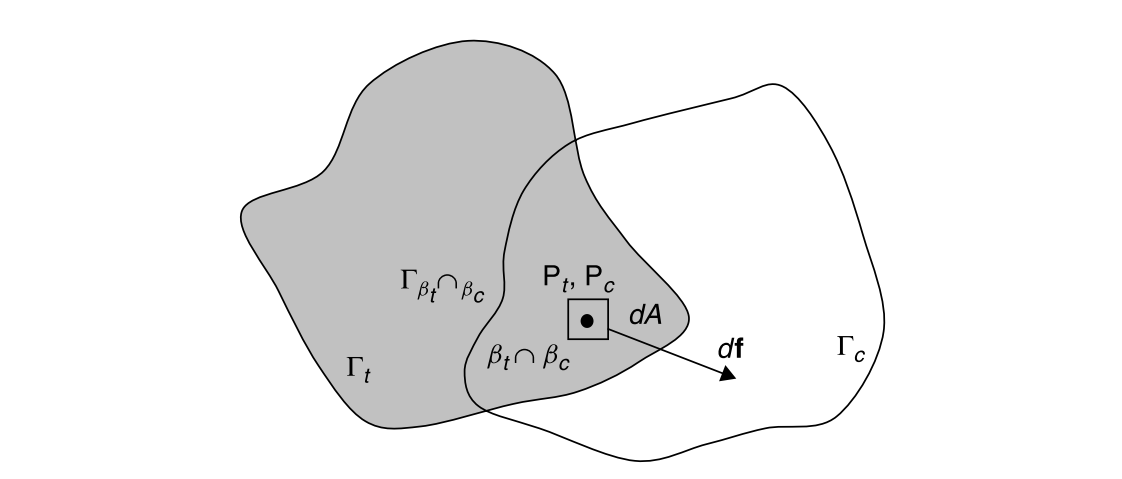
\includegraphics[width=\columnwidth]{Contact}
    \caption{Infinitesimal overlap of contractor and target body. \cite{Mun04}}
    \label{fig:contact}
\end{figure}

\bigbreak
The penetration distance $d$ for each case is given by \cite{Mun04}

\begin{equation}
    \label{eq:d}
    d=\frac{\sigma\,h}{p}\,,
\end{equation}

with applied pressure $\sigma$, element height $h$ and penalty factor $p$. The penalty factor is given by

\begin{equation}
    \label{eq:p}
    p=\alpha\,E\,,
\end{equation}

with \rm{Young's Modulus} $E$ and a constant $\alpha$ (in this paper: $\alpha=10$) to regulate penetration. Contact damping (Rayleigh damping, viscous damping) due to plastic deformation, breakage of surface asperities, etc. is given by \cite{Mun04}

\begin{equation}
    \label{eq:sigmac}
    \sigma_{\rm{C}}=4\,\xi\frac{\sqrt{p/\rho}}{h}\dot{d}\,,
\end{equation}

\addtocounter{footnote}{-1}
\stepcounter{footnote}
with damping ratio $0\leq\xi\footnotemark\leq1$ and finite element density $\rho$.  

\footnotetext{describes energy dissipation}

\section{Numerical Model Approach}
\label{sec:NumericalModelApproach}

\subsection{Software Setup}
\label{subsec:SoftwareSetup}

A \texttt{2D} input \texttt{Y} file is generated using the pre-processor \texttt{GID} \cite{GID11}. The geometry could also be imported from common \texttt{CAD} software such as \texttt{AutoCAD}.

\bigbreak
The input file is compiled using three binary files \texttt{Yf}, \texttt{m2vtk} and \texttt{m2vtk\_crack}, which constitute the \texttt{Y2D} code. The program may be obtained from the \texttt{AMCG} at Imperial College. The high performance computing (\texttt{HPC}) system at Imperial College London is applied to generate time series \texttt{.vtu} files for the simulation. 

\bigbreak
The series is analysed using the post-processing software \texttt{Hyperview} \cite{Hyp17}. For the \texttt{3D} simulation setup, which is is not considered for now, a similar approach will be applied.

\subsection{Geometry Setup}
\label{subsec:GeometrySetup}

The input file contains the model including the geometry, constraints, materials, as well as the simulation parameters. The majority of modelling parameters are adduced from the literature. A provisional list of material parameters is given in appendix table \ref{tab:matpar}. A provisional list of input file simulation parameters is provided in appendix table \ref{tab:simpar}.

\begin{figure}[h!]
    \centering
    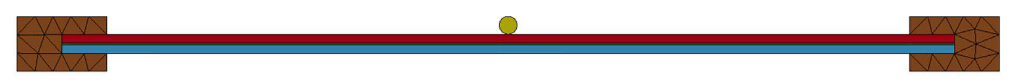
\includegraphics[width=\columnwidth]{Geometry}
    \caption{\texttt{2D} geometry of the laminated glass structure and projectile \cite{Che18}}
    \label{fig:geometry}
\end{figure}

Fig. \ref{fig:geometry} illustrates the preliminary \texttt{2D} geometric setup. The figure shows the initial state of the spherical projectile (yellow) immediately before impact on the laminated glass (impactor glass plies in red, inner glass ply in blue, inter-layer in green). The glass is fixed via a support system (brown). The support structure is not modelled for now and is replaced with no-velocity boundary conditions acting on the sides of the glass plies. 

\bigbreak
In real-world applications, the dimensions of the inter-layer are smaller compared to the glass plies. Therefore, a translational degree of freedom in the \texttt{y}-direction exists for the inter-layer. This effect will also need to be considered in this paper.

\bigbreak
Critical flaws, which cause complete structural failure, are usually found on the cut and machined glass edges \cite{Pel16}. Based on this consideration, the boundary structure layout requires special care. A project task remains to determine a realistic boundary structure to be applied.

\bigbreak
Modifications to this preliminary geometric setup will include changes to the shape of the projectile, as well as changes to the thickness of the layers. A potential consideration is to model the projectile as firearm ammunition instead of a circle (or sphere). A symmetry boundary condition may be applicable and only half of the laminate may need to be modeled.

\bigbreak
The dimensions of the glass plate is set to $2000\,{\rm{mm}}\times2000\,{\rm{mm}}$ in order to avoid anisotropic effects. The thickness of the glass plies is set to $2\,{\rm{mm}}$ and $0.76\,{\rm{mm}}$ for the inter-layer. For now, a \texttt{PVB} material is chosen for the inter-layer.

\bigbreak
The preliminary mesh for all bodies consists of triangular elements. For the \texttt{3D} model, tetrahedral elements \cite{Che18} are to be considered. The preliminary element size is $1\,{\rm{mm}}$. Necessary modifications include reducing the number of elements for the projectile, as it is not of interest for the analysis and increasing the element size for far-field mesh elements for the plies and inter-layer. Potentially, differently shaped elements are more optimal for the results. The glass and inter-layers need to consist of several element layers to enable a more precise analysis. 

\subsection{Material Parameters}
\label{subsec:MaterialParameters}

Table \ref{tab:matpar} lists the material parameters for glass, \texttt{PVB}, steel and rock. The literature provides values for most of the quantities, although they are extremely diverse in some cases. The values used in this paper are marked bold. The elastic and contact penalties are evaluated using Eq. \ref{eq:p}.

\begin{table*}
  \setlength{\tabcolsep}{2pt}
  \small
  %\flushleft
  \caption{List of Y2 input material parameter values.}
  \begin{tabular}{@{}lllll@{}}
    Property & Glass & PVB & Steel Projectile & Rock\tablefootnote{for reference}  \\\midrule
    
    Density $\rho\,\left[{\rm{kg}} / {\rm{m}}^3\right]$
    
                &$2500$ \cite{Xu10, Aba13, Che18, Ved17, Gao14}  
                
                &\begin{tabular}[t]{@{}l@{}}
                    $870$ \cite{Gao14} \\ 
                    $\bm{1100}$ \cite{Xu10, Che18, Ved17} \\
                    $1105{\rm{e}}3$ \cite{Che18}\\
                \end{tabular}
                
                & $7800$ \cite{Che18} & $2700$\\[1em]

    Young's Modulus $E\,\left[{\rm{Pa}}\right]$
    
                & \begin{tabular}[t]{@{}l@{}}
                    $\bm{7{\rm{e}}10}$ \cite{Xu10, Che18, Ved17}\\
                    $7.409{\rm{e}}10$ \cite{Gao14}\\
                    $7.41{\rm{e}}10$ \cite{Che18}\\
                    $7.5{\rm{e}}10$ \cite{Aba13}\\
                \end{tabular}
                
                & \begin{tabular}[t]{@{}l@{}}
                    $\bm{1{\rm{e}}8}$ \cite{Che18} \\
                    $2.2{\rm{e}}2$ \cite{Ved17}\\
                    $5{\rm{e}}10$ \cite{Gao14}\\
                \end{tabular}
                
                & $2{\rm{e}}11$ \cite{Che18} & $3{\rm{e}}10$ \\[1em]
                
    Poisson's Ratio $\nu$ & \begin{tabular}[t]{@{}l@{}}
                                $0.2$ \cite{Che18, Gao14} \\
                                $0.21$ \cite{Aba13} \\
                                $0.3$ \cite{Che18} \\
                                $0.22$ \cite{Xu10} \\
                                $\bm{0.23}$ \cite{Ved17}\\
                                $0.25$ \cite{Che18}
                            \end{tabular}
                          
                          & \begin{tabular}[t]{@{}l@{}}
                                $0.42$ \cite{Che18} \\
                                $0.45$ \cite{Aba13} \\
                                $0.48$ \cite{Gao14} \\
                                $0.49$ \cite{Che15} \\
                                $\bm{0.495}$ \cite{Ved17}
                            \end{tabular}
                          
                          & $0.29$ \cite{Che18} & $0.205$\\[1em]
                          
    Mass damping coefficient $\mu$\tablefootnote{Rayleigh damping, viscous damping} & $0$ & $0$ & $0$ & $0$ \\[1em]
    
    Elastic penalty term (see Eq. \ref{eq:p}) & $7{\rm{e}}11$ & $1{\rm{e}}9$ & $2.0{\rm{e}}12$  & $3.0{\rm{e}}11$\\[1em]
    
    Contact penalty (see Eq. \ref{eq:p}) & $7{\rm{e}}11$ & $1{\rm{e}}9$ & $2.0{\rm{e}}12$  & $3.0{\rm{e}}11$\\[1em]

    Mode I energy rate $G_{\rm{I}}\,\left[{\rm{J}}/{\rm{m}}^2\right]$ & 
    
    \begin{tabular}[t]{@{}l@{}}
            $\bm{10}$ \cite{Xu10}\\
            $3.9$ \cite{Che18} \\
            $4.0$ \cite{Che18}
        \end{tabular}
        
    & \begin{tabular}[t]{@{}l@{}}
            $2.8{\rm{e}}3$ \cite{Hoo17} \\
            $\bm{20}$ \cite{Che18}
        \end{tabular}  
    
    & $1.9{\rm{e}}5$ \cite{Sta00} & $20.0$\\[1em]

    Mode II energy rate $G_{\rm{II}}\,\left[{\rm{J}}/{\rm{m}}^2\right]$ & $50$ \cite{Xu10} & $2.8{\rm{e}}3$ & $1.9{\rm{e}}5$ & $100.0$ \\[1em]
    
    Mode III energy rate $G_{\rm{III}}\,\left[{\rm{J}}/{\rm{m}}^2\right]$ & $50$ \cite{Xu10} & $2.8{\rm{e}}3$ & $1.9{\rm{e}}5$ & $100.0$ \\[1em]
    
    Tensile Strength $\sigma\,\left[{\rm{Pa}}\right]$ & \begin{tabular}[t]{@{}l@{}}
            $6{\rm{e}}7$ \cite{Che15}\\
            $3{\rm{e}}7$ \cite{Che18}\\
            $\bm{3.46{\rm{e}}7}$ \cite{Che18}\\
        \end{tabular}
        
        & \begin{tabular}[t]{@{}l@{}}
            $\bm{2{\rm{e}}7}$ \cite{Zan12}\\
            $1.862{\rm{e}}7$ \cite{Che18}\\
        \end{tabular}
        
        & $1{\rm{e}}7$ \cite{Wu14} & $4{\rm{e}}6$\\[1em]
        
    Shear Strength $\tau\,\left[{\rm{Pa}}\right]$ & $17.9$ \cite{Che18} & $17.9$ \cite{Che18} & & \\[1em]
    
    Internal friction coefficient $\eta$ (Eq. \ref{eq:intfriccoeff}) & $0.1$ \cite{Che15}  & $0.7$ \cite{Kun15} & $0.15$ \cite{Sah07} & $0.6$ \\[1em]
    
    Internal cohesion $c\,\left[{\rm{Pa}}\right]$ (Eq. \ref{eq:MohrCoulomb}) & $7{\rm{e}}10$ & $2.2{\rm{e}}2$ & $2{\rm{e}}11$ & $8{\rm{e}}6$ \\[1em]
    
    Pore fluid pressure\tablefootnote{\label{notrel}not relevant for glass, \texttt{PVB} and steel} $\left[{\rm{Pa}}\right]$ & $0$ & $0$ & $0$ & $0$ \\
    
    Joint friction coefficient\textsuperscript{\ref{notrel}} & $0.6$ & $0.6$ & $0.6$ & $0.6$ \\
    
    Joint roughness coefficient $\texttt{JRC}_{\rm{0}}$ \textsuperscript{\ref{notrel}, }\tablefootnote{\label{jrc}at laboratory conditions} & $15$ & $15$ & $15$ & $15$ \\
    
    Joint compressive strength $\texttt{JCS}_{\rm{0}}$\textsuperscript{\ref{notrel}, \ref{jrc}} $\left[{\rm{MPa}}\right]$ & $120$ & $120$ & $120$ & $120$ \\
    
    Joint sample size $\left[{\rm{m}}\right]$\textsuperscript{\ref{notrel}} & $0.2$ & $0.2$ & $0.2$ & $0.2$\\[1em]
    
    Interface friction & $0.1$ \cite{Che15} & $0.62$ \cite{Fah07} & $0.44$ \cite{Fah07} & $0.6$ \\
    
    2D Problems & plane strain & & \\\bottomrule
  \end{tabular}
  \label{tab:matpar}
\end{table*}

\subsection{Problem Parameters}
\label{subsec:ProblemParameters}

\begin{table}[t]
  \caption{List of Y2D input simulation parameter values.}
  \begin{tabularx}{\columnwidth}{ll}
    Parameter                               & Value                     \\\midrule
    Maximum number of timesteps $n_{\rm{t}}$ (Eq. \ref{eq:nt})& $2{\rm{e}}6$         \\
    Current number of timesteps             & $0$                       \\
    Restart file saving frequency           & $1{\rm{e}}2$              \\
    Gravity in \texttt{X} Direction (m/s2)  & $0$                       \\
    Gravity in \texttt{Y} Direction (m/s2)  & $0$                       \\
    Gravity in \texttt{Z} Direction (m/s2)  & $-9.8$                    \\
    Timestep (s) (Eq. \ref{eq:deltat})      & $1{\rm{e}}-6$             \\
    Output frequency                        & $2{\rm{e}}3$              \\
    Current number of iterations            & $0$                       \\
    Gravity setting stage (s)               & $0$                       \\
    Load ramping stage (s)                  & $0$                       \\
    Maximum dimension (m)                   & $10$                      \\
    Maximum force (N)                       & $1{\rm{e}}6$              \\
    Maximum velocity (m/s)                  & $100$                     \\
    Maximum stress (Pa)                     & $1{\rm{e}}8$              \\
    Maximum displacement (m)                & $0.1$                     \\
    Minimum joint aperture (m)              & $1{\rm{e}}-7$             \\
    Maximum contacting couples              & $1{\rm{e}}7$              \\
    Buffer Size $b$ for NBS (m) (Eq. \ref{eq:buff})& $7.60{\rm{e}}-5$       \\
    Accuracy (bit)                          & $32$                      \\
    Joint friction model                    & {\small Coulomb}          \\
    Initial aperture correlation            & {\small roughness}        \\\bottomrule
  \end{tabularx}
  \label{tab:simpar}
\end{table}

\begin{table}[t]
  \caption{List of auxiliary parameter values (to calculate simulation parameter values).}
  \begin{tabularx}{\columnwidth}{ll}
    Parameter                               & Value                     \\\midrule
    Total minimum element volume $V_{\rm{e}}$ ($m^3$)& $1.00{\rm{e}}-07$\\
    Total minimum edge $\Delta_{\rm{min}}$ (m)& $4.13{\rm{e}}-04$       \\
    Total real simulation time $t$ (s)        & $10$                    \\
    Critical time step glass (s) (Eq. \ref{eq:deltatcrit})& $2{\rm{e}}6$\\
    Critical time step steel (s) (Eq. \ref{eq:deltatcrit})&$2{\rm{e}}6$ \\
    Critical time step \texttt{PVB} (s) (Eq. \ref{eq:deltatcrit})&$2{\rm{e}}6$   \\
    Overall Mesh size (m)                   & $2.5{\rm{e}}-4$           \\
    Mesh size projectile (m)                & $2.5{\rm{e}}-4$           \\
    Mesh size plies (m)                     & $2.5{\rm{e}}-4$           \\
    Mesh size inter-layer (m)               & $2.5{\rm{e}}-4$           \\\bottomrule
  \end{tabularx}
  \label{tab:simpar}
\end{table}

\bigbreak
The radius of the steel sphere (or circle) is set to $2.5\,{\rm{mm}}$. The critical time step \cite{Far19}\footnote{\label{DEMPlus} for inquiries concerning this reference please contact the \texttt{AMCG} at Imperial College London} is set accordingly to

\begin{equation}
\label{eq:deltatcrit}
\Delta t_{\rm{crit}}=\sqrt{\frac{V_{\rm{e}}\footnotemark\,\rho\footnotemark}{p}}=\sqrt{\frac{0.000413\cdot7.8\cdot10^3}{4\cdot{10}^{11}}}{\rm{s}}\,.
\end{equation}

\addtocounter{footnote}{-2}
\stepcounter{footnote}
\footnotetext{volume  $\left({\rm{in}}\,{\rm{m}}^3\right)$ of the smallest finite element, without units}
\stepcounter{footnote}
\footnotetext{density $\left({\rm{in}}\,{\rm{kg}}/{\rm{m}}^3\right)$ of the material of the smallest finite element, without units}

The acceptable time step $\Delta t$ is given by

\begin{equation}
    \label{eq:deltat}
    \Delta t= \floor{\Delta t_{\rm{crit}}} = 3\rm{e}-6{\rm{s}}\,,
\end{equation},

where $\floor{\,}$ denotes the floor operator. To simulate real time $t=10\,{\rm{s}}$, the maximum number of time steps required \cite{Far19}\textsuperscript{\ref{DEMPlus}} is given by

\begin{equation}
    \label{eq:nt}
    n_{\rm{t}}=\frac{t}{\Delta t}=\frac{10\,{\rm{s}}}{3\,{\rm{e}}-6\,{\rm{s}}}=1{\rm{e}}6\,.
\end{equation}

\subsection{Verification}
\label{subsec:Verification}

Meeting specified accuracy standards \cite{Sto15} requires verification of the numerical model by use of data from numerical experiments. Physical experiments involving the breakage of glass by projectiles or shock blasts require special safety arrangements. Air blast impact experiments are being conducted outdoors by service company \texttt{Jabisupra} \cite{Jab16} in cooperation with Imperial College London. The company is active in the field of envelope security and specialises in protecting infrastructure from certain threats. The data from \texttt{Jabisupra} is not expected to yet be ready and applicable for this project. Many other researchers have already conducted impact experiments in the past and a majority of the findings from these experiments are likely to be applicable to verify the model for this project.

\bigbreak
Dynamic impact on laminated glass comprises hard and soft body impact \cite{Moh17}. Hard body impact such as ballistic impact \cite{Bra10} causes minimal deformation to the projectile, while soft body impact such as bird impact \cite{Moh17} causes the projectile to undergo extensive deformation.

\bigbreak
Relevant parameters of the impact projectile include the normal velocity \cite{Gra98, Kar14, Dar13, Wu14}, the mass \cite{Kar14, Dar13}, the angle \cite{Gra98, Kar14, Dar13}, the shape \cite{Dar13} and the size \cite{Wu14}. Relevant parameters for the outer glass ply include its dimensions \cite{Wan18}, its mass, the support conditions \cite{Wan18} and the make-up \cite{Wan18}. For the inter-layer, the material \cite{Moh18, Wan18, Mon04}, thickness \cite{Ji98, Kar14, Wan18} and temperature \cite{Moh18, Zha19} are relevant.

\bigbreak
Low velocity ($\approx 20\,\mathrm{m}/\mathrm{s}$) hard impact experiments include the use of projectiles in form of road construction chippings \cite{Gra98}, ballistics \cite{Mon04}, drop-down weights \cite{Che15, Mil12, Wan18}, aluminum projectiles \cite{Mil12} and steel balls \cite{Beh99, Flo98, Wan18}. High velocity (around $180\, {\rm{m}}/{\rm{s}}$) soft impact experiments include the use of silicon rubber projectiles \cite{Moh17} and gas guns \cite{Moh18}.

\bigbreak
Wang et al \cite{Wan18} found that the panel size had an inferior effect on the breakage resistance \cite{Wan18}. Similarly, Monteleone et al \cite{Mon04} found that only a local area of the ply around the impact absorbed the impact energy for high velocities.

\bigbreak
Karunarathna \cite{Kar14} found that impact velocity and plate thickness contributed significantly towards the impact resistance, compared to impact mass and inter-layer thickness. Wang et al \cite{Wan18} found an increased inter-layer thickness to have a negative effect on energy absorption. Liu et al \cite{Liu16} established that the inter-layer thickness did not contribute towards energy absorption. Behr and Kremer \cite{Beh99} found an increased inter-layer thickness to better protect the inner ply. Kim et al \cite{Kim16} numerically optimised the \texttt{PVB} inter-layer constitution to prevent all damage to the inner glass ply.

\bigbreak
Liu et al \cite{Liu16} numerically investigated the optimisability of the inter-layer in terms of energy absorption by simulating the impact of a human head. Zhang et al \cite{Zha19} investigated the influence of temperature on the inter-layer and found that a hybrid \texttt{TPU}/\texttt{SGP}/\texttt{TPU} inter-layer performed best over the entire range of tested temperatures.

\section{Discussion}

The results show...

\begin{acks}
The authors would like to thank the \texttt{AMCG} for supporting this project and the course director Dr Gerard Gorman\footnote{g.gorman@imperial.ac.uk, Imperial College London, Department of Earth and Science} for enabling this research.
\end{acks}

\medskip
\printbibliography

%\appendix
%\setcounter{table}{0}
%\renewcommand{\thetable}{\Alph{table}}

%\section{Material Parameters}
%\label{sec:MaterialParameters}

%\section{Simulation Parameters}
%\label{sec:SimulationParameters}

%\newpage
%
%\begin{table}[h!]
%  \centering
%  \begin{tabular}{ll}
%    Parameter               & Description                       \\\midrule  
%    
%    \texttt{/YD/YDC/MCSTEP} & Maximum number of timesteps       \\
%    \texttt{/YD/YDC/NCSTEP} & Current number of timesteps       \\
%    \texttt{/YD/YDC/ISAVE}  & Restart file saving frequency     \\
%    \texttt{/YD/YDC/DCGRAX} & Gravity in \texttt{X} Direction   \\
%    \texttt{/YD/YDC/DCGRAY} & Gravity in \texttt{Y} Direction   \\
%    \texttt{/YD/YDC/DCGRAZ} & Gravity in \texttt{Z} Direction   \\
%    \texttt{/YD/YDC/DCSTEC} & Size of timestep                  \\
%    \texttt{/YD/YDC/DCTIME} & Current time                      \\
%    \texttt{/YD/YDC/DCURELX}& Not specified                     \\
%    \texttt{/YD/YDC/INITER} & Not specified                     \\
%    \texttt{/YD/YDC/ICOUTF} & Output frequency                  \\
%    \texttt{/YD/YDC/ICOUTI} & Current number of iterations      \\
%    \texttt{/YD/YDC/DCSIZC} &                                   \\
%    \texttt{/YD/YDC/DCSIZF} &                                   \\
%    \texttt{/YD/YDC/DCSIZS} &                                   \\
%    \texttt{/YD/YDC/DCSIZV} &                                   \\
%    \texttt{/YD/YDC/DCSIZD} &                                   \\
%    \texttt{/YD/YDC/DCSIZA} &                                   \\
%    \texttt{/YD/YDC/DCSTEC} &                                   \\
%    \texttt{/YD/YDC/DCTIME} &                                   \\
%    \texttt{/YD/YDC/DCRMPT} &                                   \\
%    \texttt{/YD/YDC/DCGRST} &                                   \\
%    \texttt{/YD/YDC/ICSAVF} &                                   \\
%    \texttt{/YD/YDC/ICOUTP} &                                   \\
%    \texttt{/YD/YDC/ICFMTY} &                                   \\
%    \texttt{/YD/YDC/ICIATY} &                                   \\\bottomrule
%  \end{tabular}
%  \caption{List of preliminary Y2D input simulation parameter values}
%  \label{tab:inpar}
%\end{table}

\end{document}


% Tables, Figures and Equations

%%%%%%%%%%%%%%%%%%%%%%%%%%%%%%%%%%%%%%%%%%%%%%%%%
%TABLES%
%%%%%%%%%%%%%%%%%%%%%%%%%%%%%%%%%%%%%%%%%%%%%%%%%
%\section{Tables}
%
%The ``\texttt{acmart}'' document class includes the ``\texttt{booktabs}''
%package --- \url{https://ctan.org/pkg/booktabs} --- for preparing
%high-quality tables.
%
%Table captions are placed {\itshape above} the table.
%
%Because tables cannot be split across pages, the best placement for
%them is typically the top of the page nearest their initial cite.  To
%ensure this proper ``floating'' placement of tables, use the
%environment \textbf{table} to enclose the table's contents and the
%table caption.  The contents of the table itself must go in the
%\textbf{tabular} environment, to be aligned properly in rows and
%columns, with the desired horizontal and vertical rules.  Again,
%detailed instructions on \textbf{tabular} material are found in the
%\textit{\LaTeX\ User's Guide}.
%
%Immediately following this sentence is the point at which
%Table~\ref{tab:freq} is included in the input file; compare the
%placement of the table here with the table in the printed output of
%this document.
%
%\begin{table}
%  \caption{Frequency of Special Characters}
%  \label{tab:freq}
%  \begin{tabular}{ccl}
%    \toprule
%    Non-English or Math&Frequency&Comments\\
%    \midrule
%    \O & 1 in 1,000& For Swedish names\\
%    $\pi$ & 1 in 5& Common in math\\
%    \$ & 4 in 5 & Used in business\\
%    $\Psi^2_1$ & 1 in 40,000& Unexplained usage\\
%  \bottomrule
%\end{tabular}
%\end{table}
%
%To set a wider table, which takes up the whole width of the page's
%live area, use the environment \textbf{table*} to enclose the table's
%contents and the table caption.  As with a single-column table, this
%wide table will ``float'' to a location deemed more
%desirable. Immediately following this sentence is the point at which
%Table~\ref{tab:commands} is included in the input file; again, it is
%instructive to compare the placement of the table here with the table
%in the printed output of this document.
%
%\begin{table*}
%  \caption{Some Typical Commands}
%  \label{tab:commands}
%  \begin{tabular}{ccl}
%    \toprule
%    Command &A Number & Comments\\
%    \midrule
%    \texttt{{\char'134}author} & 100& Author \\
%    \texttt{{\char'134}table}& 300 & For tables\\
%    \texttt{{\char'134}table*}& 400& For wider tables\\
%    \bottomrule
%  \end{tabular}
%\end{table*}
%
%%%%%%%%%%%%%%%%%%%%%%%%%%%%%%%%%%%%%%%%%%%%%%%%%
%%%%%%%%%%%%%%%%%%%%%%%%%%%%%%%%%%%%%%%%%%%%%%%%%
%%%%%%%%%%%%%%%%%%%%%%%%%%%%%%%%%%%%%%%%%%%%%%%%%
%Equations%
%%%%%%%%%%%%%%%%%%%%%%%%%%%%%%%%%%%%%%%%%%%%%%%%%
%\section{Math Equations}
%You may want to display math equations in three distinct styles:
%inline, numbered or non-numbered display.  Each of the three are
%discussed in the next sections.
%
%\subsection{Inline (In-text) Equations}
%A formula that appears in the running text is called an inline or
%in-text formula.  It is produced by the \textbf{math} environment,
%which can be invoked with the usual
%\texttt{{\char'134}begin\,\ldots{\char'134}end} construction or with
%the short form \texttt{\$\,\ldots\$}. You can use any of the symbols
%and structures, from $\alpha$ to $\omega$, available in
%\LaTeX~\cite{Lamport:LaTeX}; this section will simply show a few
%examples of in-text equations in context. Notice how this equation:
%\begin{math}
%  \lim_{n\rightarrow \infty}x=0
%\end{math},
%set here in in-line math style, looks slightly different when
%set in display style.  (See next section).
%\subsection{Display Equations}
%A numbered display equation---one set off by vertical space from the
%text and centered horizontally---is produced by the \textbf{equation}
%environment. An unnumbered display equation is produced by the
%\textbf{displaymath} environment.
%Again, in either environment, you can use any of the symbols and
%structures available in \LaTeX\@; this section will just give a couple
%of examples of display equations in context.  First, consider the
%equation, shown as an inline equation above:
%\begin{equation}
%  \lim_{n\rightarrow \infty}x=0
%\end{equation}
%Notice how it is formatted somewhat differently in
%the \textbf{displaymath}
%environment.  Now, we'll enter an unnumbered equation:
%\begin{displaymath}
%  \sum_{i=0}^{\infty} x + 1
%\end{displaymath}
%and follow it with another numbered equation:
%\begin{equation}
%  \sum_{i=0}^{\infty}x_i=\int_{0}^{\pi+2} f
%\end{equation}
%just to demonstrate \LaTeX's able handling of numbering.
%%%%%%%%%%%%%%%%%%%%%%%%%%%%%%%%%%%%%%%%%%%%%%%%%
%%%%%%%%%%%%%%%%%%%%%%%%%%%%%%%%%%%%%%%%%%%%%%%%%
%%%%%%%%%%%%%%%%%%%%%%%%%%%%%%%%%%%%%%%%%%%%%%%%%
%Figures%
%%%%%%%%%%%%%%%%%%%%%%%%%%%%%%%%%%%%%%%%%%%%%%%%%
%\section{Figures}
%\begin{figure}[h]
%  \centering
%  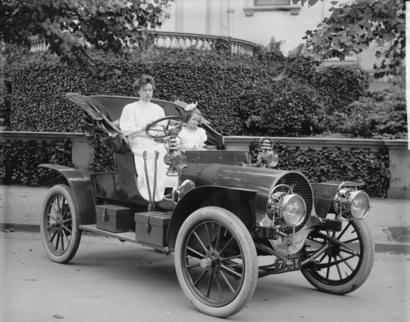
\includegraphics[width=\linewidth]{sample-franklin}
%  \caption{1907 Franklin Model D roadster. Photograph by Harris \&
%    Ewing, Inc. [Public domain], via Wikimedia
%    Commons. (\url{https://goo.gl/VLCRBB}).}
%  \Description{The 1907 Franklin Model D roadster.}
%\end{figure}
%Figure captions are placed {\itshape below} the figure.
%\subsection{The ``Teaser Figure''}
%A ``teaser figure'' is an image, or set of images in one figure, that
%are placed after all author and affiliation information, and before
%the body of the article, spanning the page. If you wish to have such a
%figure in your article, place the command immediately before the
%\texttt{\maketitle} command:
%\begin{verbatim}
%  \begin{teaserfigure}
%    \includegraphics[width=\textwidth]{sampleteaser}
%    \caption{figure caption}
%    \Description{figure description}
%  \end{teaserfigure}
%\end{verbatim}
%%%%%%%%%%%%%%%%%%%%%%%%%%%%%%%%%%%%%%%%%%%%%%%%%
%%%%%%%%%%%%%%%%%%%%%%%%%%%%%%%%%%%%%%%%%%%%%%%%%